\documentclass[12pt,a4paper,english]{article}
\usepackage{times}
\usepackage[utf8]{inputenc}
\usepackage{babel,textcomp}
\usepackage{mathpazo}
\usepackage{mathtools}
\usepackage{amsmath,amssymb}
\usepackage{ dsfont }
\usepackage{listings}
\usepackage{graphicx}
\usepackage{float}
\usepackage{subfig} 
\usepackage[colorlinks]{hyperref}
\usepackage[usenames,dvipsnames,svgnames,table]{xcolor}
\usepackage{textcomp}
\definecolor{listinggray}{gray}{0.9}
\definecolor{lbcolor}{rgb}{0.9,0.9,0.9}
\lstset{backgroundcolor=\color{lbcolor},tabsize=5,rulecolor=,language=matlab,basicstyle=\scriptsize,upquote=true,aboveskip={1.5\baselineskip},columns=fixed,numbers=none,showstringspaces=false,extendedchars=false,breaklines=true,
prebreak=\raisebox{0ex}[0ex][0ex]{\ensuremath{\hookleftarrow}},frame=single,showtabs=false,showspaces=false,showstringspaces=false,identifierstyle=\ttfamily,keywordstyle=\color[rgb]{0.9,0.9,0.9},commentstyle=\color[rgb]{0.133,0.545,0.133},stringstyle=\color[rgb]{0.627,0.126,0.941},literate={å}{{\r a}}1 {Å}{{\r A}}1 {ø}{{\o}}1}

% Use for references
%\usepackage[sort&compress,square,comma,numbers]{natbib}
%\DeclareRobustCommand{\citeext}[1]{\citeauthor{#1}~\cite{#1}}

% Fix spacing in tables and figures
%\usepackage[belowskip=-8pt,aboveskip=5pt]{caption}
%\setlength{\intextsep}{10pt plus 2pt minus 2pt}

% Change the page layout
%\usepackage[showframe]{geometry}
\usepackage{layout}
\setlength{\hoffset}{-0.4in}  % Length left
%\setlength{\voffset}{-0.4in}  % Length on top
\setlength{\textwidth}{460pt}  % Width /597pt
%\setlength{\textheight}{640pt}  % Height /845pt
%\setlength{\footskip}{25pt}

\newcommand{\VEV}[1]{\langle#1\rangle}
\title{FYS4565 - Obligatory exercise:\\ Emittance preservation techniques in a linear accelerator}
\date{}
\author{ Kristoffer Langstad \footnote{GitHub-repository: \url{https://github.com/krilangs/FYS4565/tree/master}}\\ \textit{krilangs@uio.no}}

\begin{document}%\layout
\maketitle
\section*{Exercises}
\label{sect:Exercises}
\subsection*{Theory}
\label{subsect:Theory}
\subsubsection*{1)}
The (geometric) emittance, $\varepsilon$, is defined as a space area. The normalized emittance, $\varepsilon$, is defined as the emittance which is preserved while the beam is accelerated when there are source of emittance growth. This normalized emittance is given as:
\begin{equation}
\label{eq:norm_em}
\varepsilon_N=\beta\gamma\varepsilon
\end{equation}
$\beta$ and $\gamma$ are the relativistic functions normalized velocity and the Lorentz factor, respectively. Geometric emittance is only constant when there is no acceleration involved with the beam, while normalized emittance does not change due to acceleration.

\subsubsection*{2)}
For a beam with N number of particles and phase space ${x_n,x_n^{\prime}}$, the Twiss parameters are given as:
\begin{align}
\beta &= \frac{<x_n^2>}{\varepsilon}\\
\alpha &= -\frac{1}{2}\beta=-\frac{<x_nx_n^{\prime}>}{\varepsilon}\\
\gamma &= \frac{1+\alpha^2}{\beta}=\frac{<{x_n^{\prime}}^2>}{\varepsilon}
\end{align} 
The geometric emittance is given as:
\begin{equation}
\varepsilon= \sqrt{<x_n^2><{x_n^{\prime}}^2>-<x_nx_n^{\prime}>^2}
\end{equation}

\subsection*{Emittance growth}
\label{subsect:Emittance}
The script for running the exercises in this section is \textbf{project\_part1.m}.
\subsubsection*{1)}
Run script and track a beam with \textbf{runMADX()} gives the following output:
\begin{lstlisting}
Running MADX...   ++++++++++++++++++++++++++++++++++++++++++++
+     MAD-X 5.05.02  (64 bit, Windows)     +
+ Support: mad@cern.ch, http://cern.ch/mad +
+ Release   date: 2019.07.25               +
+ Execution date: 2020.04.08 15:37:12      +
++++++++++++++++++++++++++++++++++++++++++++
OPTION, ECHO = FALSE, TWISS_PRINT = FALSE, INFO = FALSE;

initial->betx      =        3.410060363 ;
initial->bety      =        0.590010444 ;
initial->alfx      =       -2.404092556 ;
initial->alfy      =        0.415957363 ;
emit_x             =          5.11e-009 ;
emit_y             =          5.11e-009 ;

GXPLOT-X11  1.50 initialized 

plot number =            1 
plot number =            2 
enter TRACK module
one pass is on
exit TRACK module


Number of warnings: 0

++++++++++++++++++++++++++++++++++++++++++++
+          MAD-X finished normally         +
++++++++++++++++++++++++++++++++++++++++++++
Done.
\end{lstlisting}
This is to show that the program works as wanted.

\subsubsection*{2)}
Load the initial beam characterized by the 6D phase space distribution ($x,x^{\prime},y,y^{\prime}, z, \Delta E/E$). The three first values for each of the 6D phase space parameters are printed to show the program works:
\begin{lstlisting}
Initial beam:
-3.372303e-05 9.786400e-05 1.370667e-04 -5.637760e-06 1.168475e-04 9.629966e-05 
-3.942910e-05 8.925327e-05 1.275999e-04 -3.026930e-05 6.234654e-05 -5.830864e-05 
3.634007e-06 -1.178952e-05 1.350098e-06 -3.673267e-03 -4.841775e-03 1.045882e-02
\end{lstlisting}

\subsubsection*{3)}
Calculate the rms normalized emittance of the input beam from th phase space distribution. The geometric emittance is calculated to: 
\[\varepsilon_x=5.108212e-09\quad \varepsilon_y=5.105969e-09\]
The normalized emittance is calculated to:
\[\varepsilon_{N,x}=9.996502e-06\quad \varepsilon_{N,y}=9.992112e-06\]
This is the answers that we expected to get as they coincide with the input parameters ($10\mu m$).

\subsubsection*{4)}
The Twiss parameters for the input beam are calculated to give:
\begin{align*}
\alpha_x&=-2.416237,\quad \beta_x=3.414410\\
\alpha_y&=0.4237378,\quad \beta_y=0.5949598
\end{align*}
These calculated Twiss parameters are around the expected values of the MADX output of the FODO-matched solution with an expected relative error of around $1/\sqrt{N}$:
\begin{lstlisting}
initial->betx      =        3.410060363 ;
initial->bety      =        0.590010444 ;
initial->alfx      =       -2.404092556 ;
initial->alfy      =        0.415957363 ;
\end{lstlisting}

\subsubsection*{5)}
In Figure \ref{fig:beam_orbit} we see the beam position monitor (BPM) orbit ($\overline{x},\overline{y}$ vs. $s$). This BPM system determines the position of the beam, which is needed due to that the beam trajectory may be deflected from the pipe center.

\begin{figure}[htbp!]
	\centering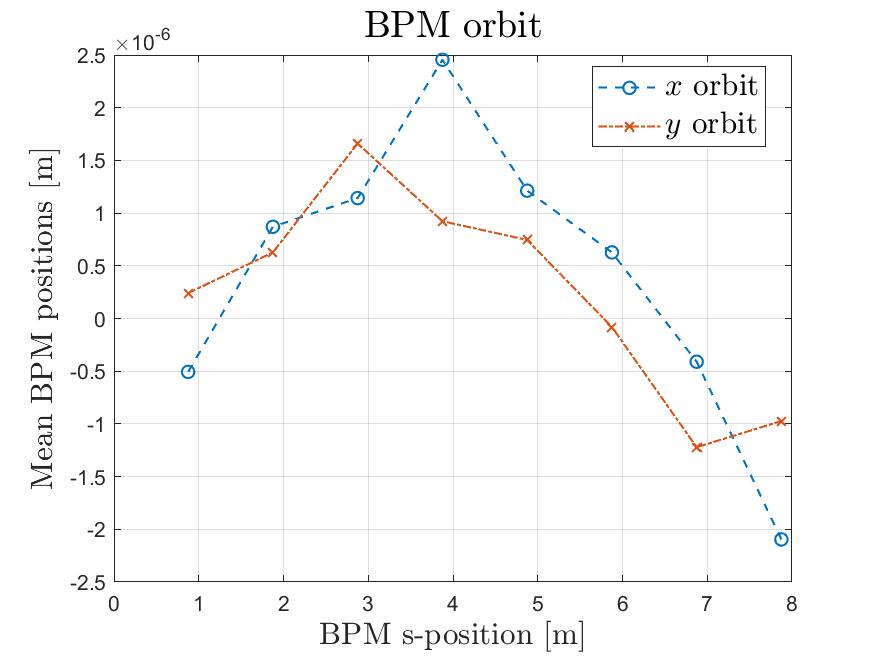
\includegraphics[width=0.65\linewidth, height=0.55\linewidth]{orbit.jpg}
	\caption{BPM orbit: $\overline{x},\overline{y}$ vs. $s$ . \label{fig:beam_orbit}}
\end{figure} 

\subsubsection*{6)}
Introduce quadrupole misalignments with a 1mm rms offset in both directions. The new BPM orbit is seen in Figure \ref{fig:mis_beam_orbit}. The mean BPM positions vary a lot more when quadrupole misalignments are introduced compared to without.

\begin{figure}[htbp!]
	\centering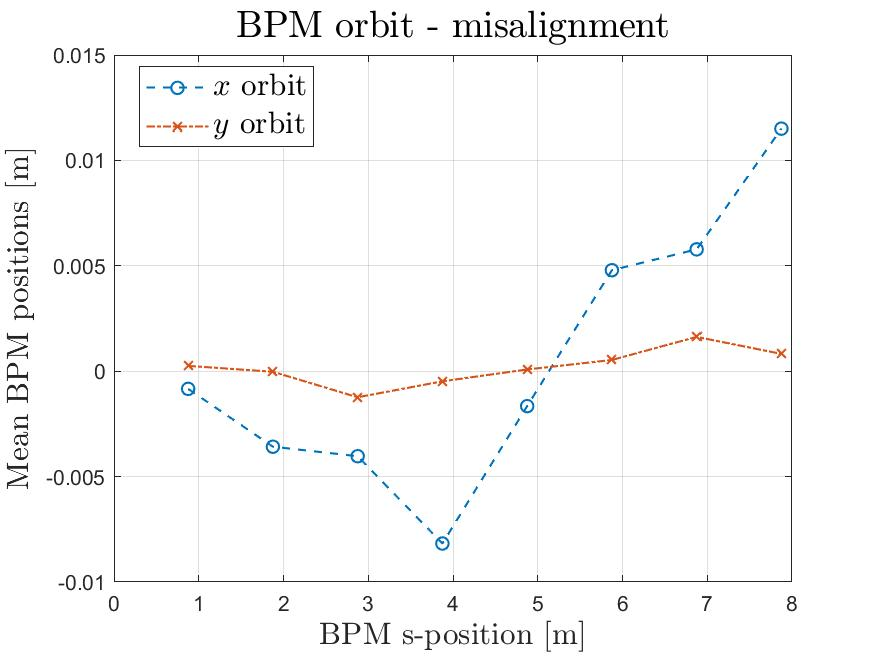
\includegraphics[width=0.65\linewidth, height=0.55\linewidth]{orbit_mis.jpg}
	\caption{BPM orbit with a 1 mm rms offset quadrupole misalignment in both directions: $\overline{x},\overline{y}$ vs. $s$. \label{fig:mis_beam_orbit}}
\end{figure} 

\subsubsection*{7)}
The dispersion function, $D(s)$, of an accelerator beam line is defined as the local sensitivity of the beam trajectory, $x(s)$, to a relative energy error $\Delta E/E$:
\begin{equation}
D(s)=\frac{x(s)}{\Delta E/E}
\end{equation}
This is calculated by first tracking a beam with the nominal energy and then by tracking a beam with slightly different energy. In Figure \ref{fig:dispersion} we see a plot of this dispersion function difference between the two beams in both directions.

\begin{figure}[htbp!]
	\centering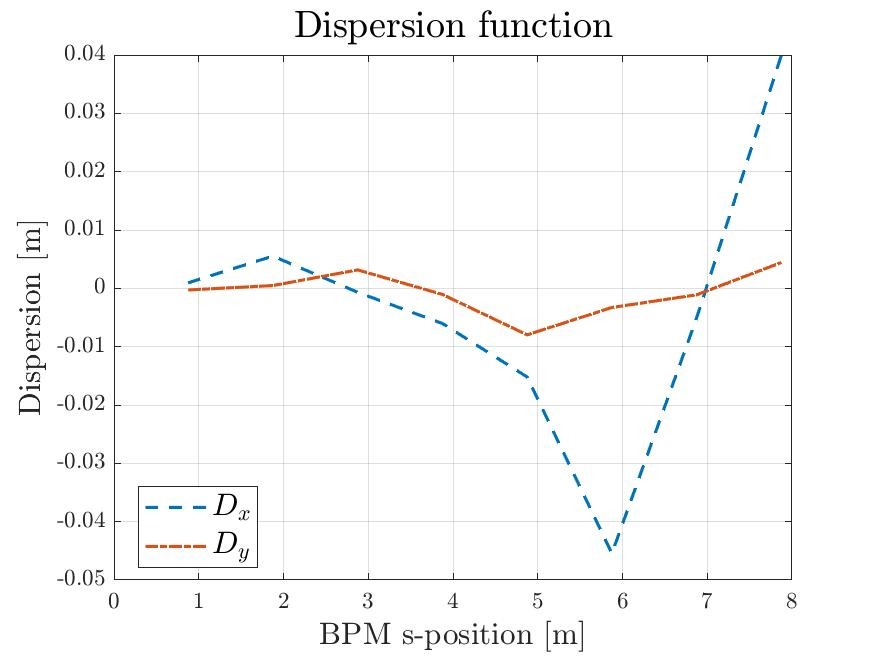
\includegraphics[width=0.65\linewidth, height=0.55\linewidth]{dispersion.jpg}
	\caption{Plot of the dispersion function as a function of the BPM s-position. \label{fig:dispersion}}
\end{figure} 

\subsubsection*{8)}
Here we set the energy spread of the input beam to zero. In Figure \ref{fig:em_growth} we see a plot of the relative emittance growth from the start of the lattice to the end of the lattice as a function of quadrupole misalignment.

\begin{figure}[htbp!]
	\centering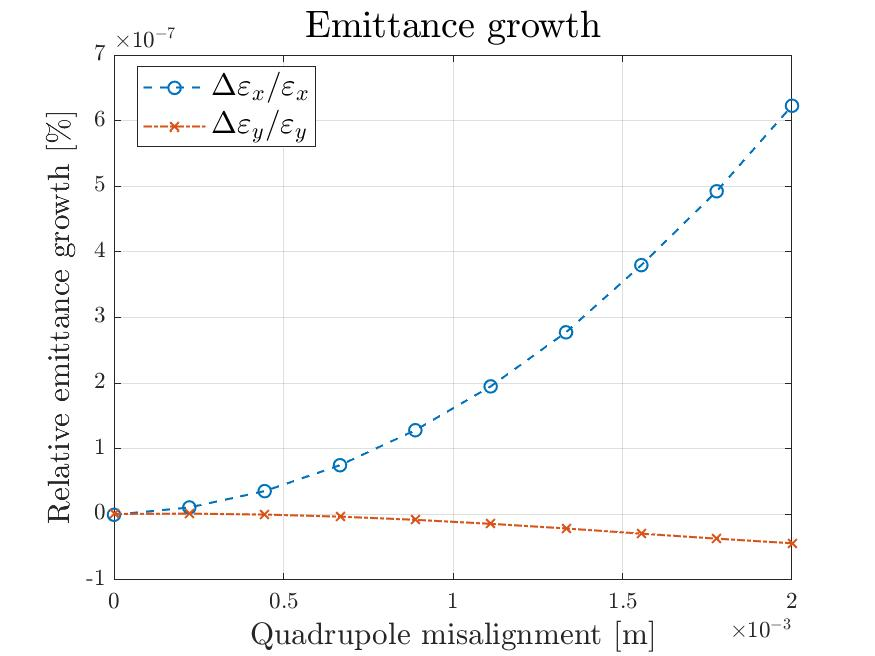
\includegraphics[width=0.65\linewidth, height=0.55\linewidth]{growth.jpg}
	\caption{Relative emittance growth from the start of the lattice to the end of the lattice as a function of quadrupole misalignment. \label{fig:em_growth}}
\end{figure} 
\newpage
\subsubsection*{9)}
Here we set the energy spread of the input beam to 1\%. In Figure \ref{fig:em_growth_spread} we see a plot of the relative emittance growth from the start of the lattice to the end of the lattice as a function of quadrupole misalignment with the small energy spread.

\begin{figure}[htbp!]
	\centering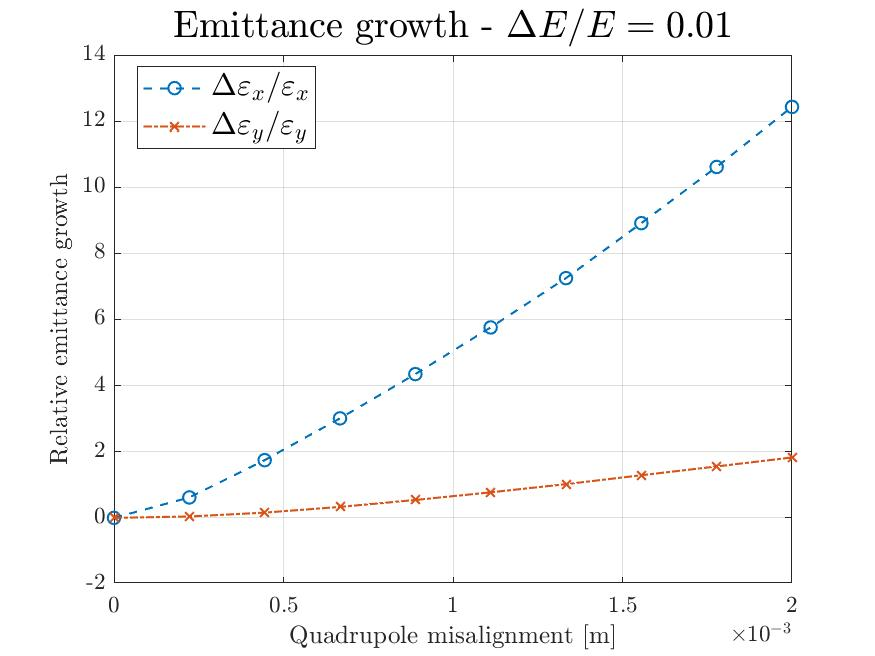
\includegraphics[width=0.65\linewidth, height=0.55\linewidth]{growth_spread.jpg}
	\caption{Relative emittance growth from the start of the lattice to the end of the lattice as a function of quadrupole misalignment with a small energy spread (1\%). \label{fig:em_growth_spread}}
\end{figure} 

\subsubsection*{10)}
For 0\% energy spread, the relative emittance growth does not change that much, increases up till only around $6\cdot10^{-7}$\%, in the lattice as the quadrupole misalignment increases. In the x-direction the emittance growth increases almost exponential, while in the y-direction it decreases a little. For 1\% energy spread, the relative emittance growth increases much more, up till almost 13\%, in the lattice as the quadrupole misalignment increases. Here the emittance growth in the x-direction is more linear, and now it increases also a little in the y-direction as well. The emittance can be seen as the area of the phase space of the position and momentum. So when there is a higher energy spread, the bigger the area becomes. This seems to be reasonable since when a particle has higher energy, it also has a higher momentum leading to a larger distance covered by the particle. So a larger energy spread should lead to a higher emittance.	

\subsubsection*{11)}
Change the quad strength $k$ of the FODO-cells by $k\in[0.8,1.0,1.2]$, and recalculate the emittance growth with a small energy spread as earlier. In Figure \ref{fig:quad_strength} we see how the emittance growth behaves in the lattice as function of quadrupole misalignment when we change the quad strength. There we see that as the quad strength increases, the higher is the emittance growth increase as the quadrupole misalignment increases. The quadrupole strength has an affect as a bending force term that increase linearly with the transverse displacement from the ideal trajectory, and has a focusing effect on the beam. This bending force term is one of the multipole terms in the magnetic field around the beam, which affects the path of the particles in the beam. This is used for beam steering in the accelerator for linear beam optics.

\begin{figure}[htbp!]
	\centering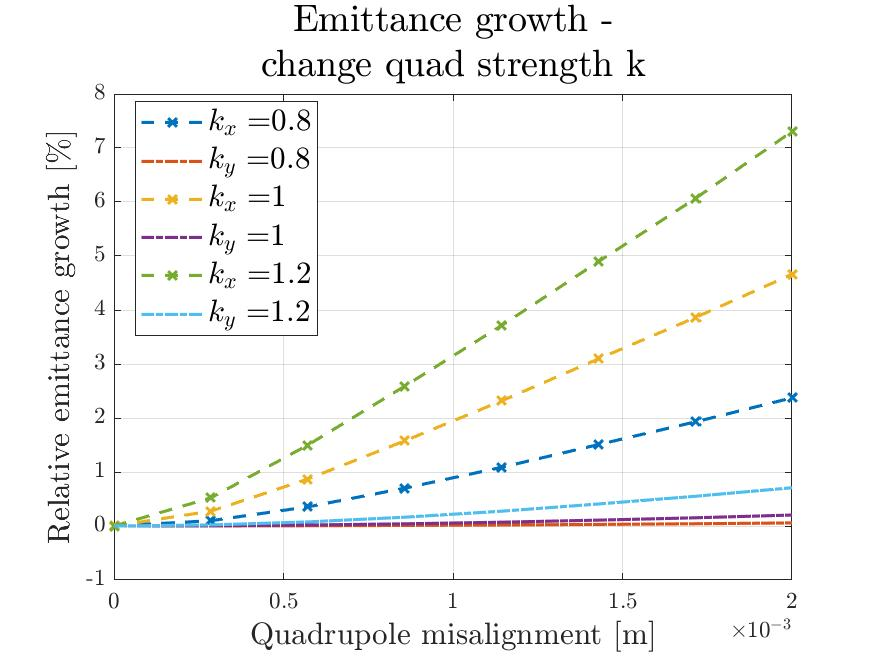
\includegraphics[width=0.65\linewidth, height=0.55\linewidth]{growth_spread_k.jpg}
	\caption{Emittance growth as function of quadrupole misalignment as we change the quad strength and with a small energy spread. \label{fig:quad_strength}}
\end{figure} 

\newpage
\subsection*{Beam-based correction}
\label{subsect:Beam correction}
The script for running the exercises in this section is \textbf{project\_part2.m}. Assume noise-free/ideal BPMs giving $\omega_0=0$, and use energy spread of 1\%. Only study the motion in the x-plane.
\subsubsection*{1)}
To steer the beam into the centre of each BPM one can add 1-to-1 correction. This is done to mitigate the growth of the centroid envelope due to quadrupole kicks. This correction is added by calculating the corrector-to-BPM response matrix. In Figure \ref{fig:1-to-1_orbit} we see a plot of the BPM orbits for both the uncorrected and 1-to-1 corrected steering. There we see that the 1-to-1 corrected BPM orbit changes a lot less (actually not at all by eye) than the uncorrected BPM orbit.

\begin{figure}[htbp!]
	\centering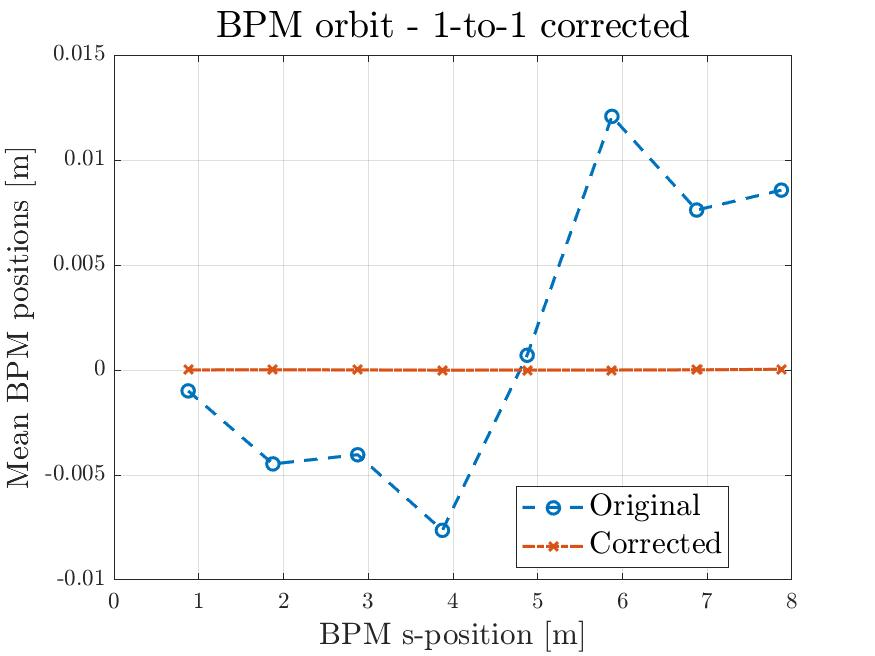
\includegraphics[width=0.65\linewidth, height=0.55\linewidth]{1-to-1-orbits.jpg}
	\caption{BPM orbits of the beam for uncorrected and 1-to-1 corrected BPM orbits. \label{fig:1-to-1_orbit}}
\end{figure} 
\newpage
\subsubsection*{2)}
In Figure \ref{fig:em_growth_1to1} we see a plot of how the emittance growth behaves as a function of the quadrupole misalignment for both uncorrected and 1-to-1 corrected BPM orbits. As before we see that for the uncorrected BPM orbit, the emittance growth increases almost linearly as the quadrupole misalignments increases. The emittance growth for 1-to-1 corrected BPM orbit is more or less constant by eye (actually it has small deviations close to 0\%) as a function of quadrupole misalignment. So the 1-to-1 correction does improve the orbit, and the emittance growth, of the beam by steering the beam into the BPM centers by using the response matrix.

\begin{figure}[htbp!]
	\centering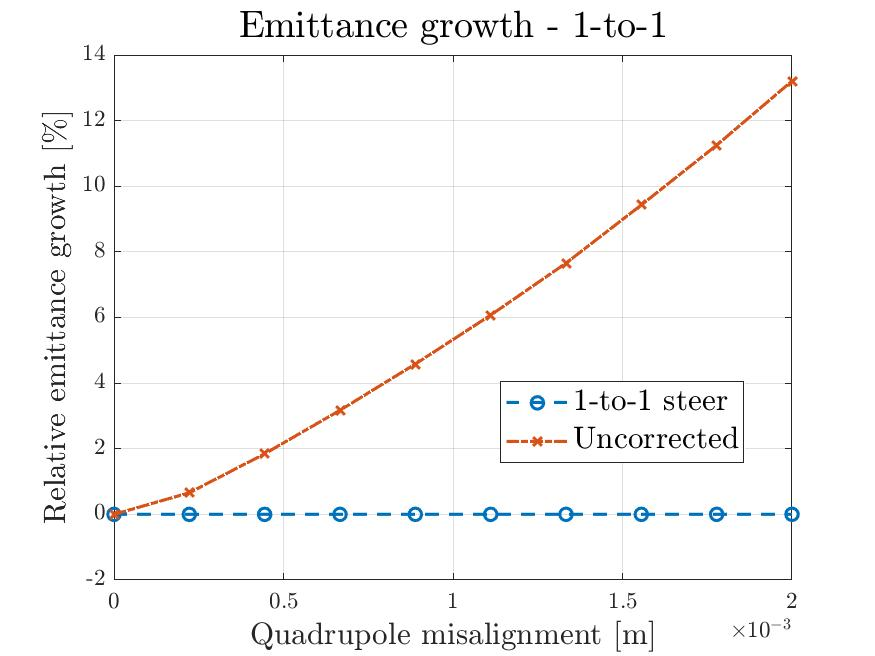
\includegraphics[width=0.65\linewidth, height=0.5\linewidth]{growth_1-to-1.jpg}
	\caption{Relative emittance growth from the start of the lattice to the end of the lattice as a function of quadrupole misalignment for both uncorrected and 1-to-1 corrected BPM orbits. \label{fig:em_growth_1to1}}
\end{figure} 

\subsubsection*{3)}
Then we introduce 1 mm rms BPM misalignments and plot the BPM orbits of the uncorrected and 1-to-1 corrected steering again. This is seen in Figure \ref{fig:1-to-1_BPM_orbit}. The BPM misalignments changes the uncorrected orbit a little compared to the uncorrected orbit in Figure \ref{fig:1-to-1_orbit} without BPM misalignments. The 1-to-1 corrected BPM orbit does not seem to change, and is still more or less constant with mean BPM position at 0. This seems right, since the 1-to-1 correction always tries to steer the orbit through the centers of the BPMs.

\begin{figure}[htbp!]
	\centering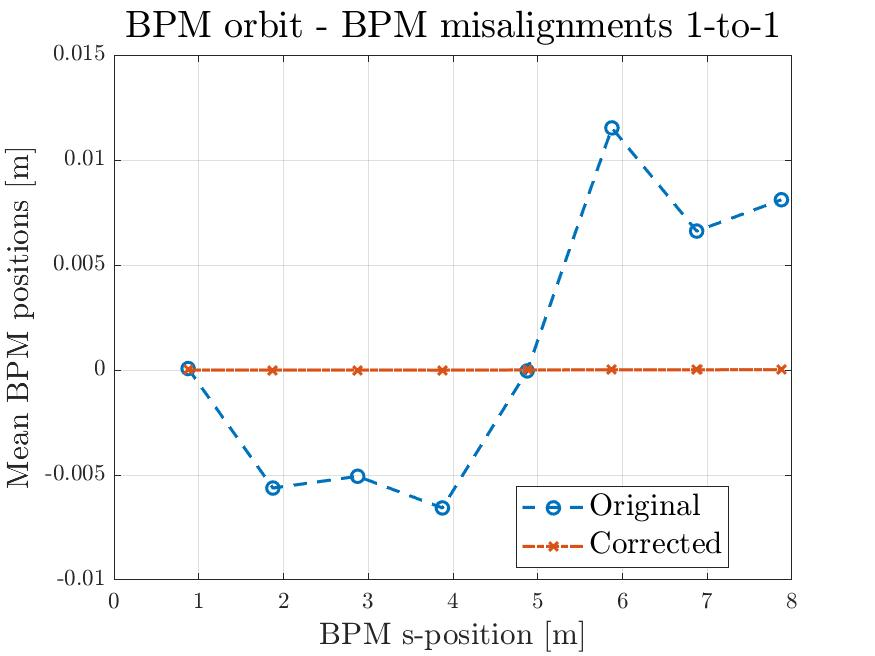
\includegraphics[width=0.65\linewidth, height=0.5\linewidth]{1-to-1-orbits_BPM.jpg}
	\caption{BPM orbits of the beam for uncorrected and 1-to-1 corrected BPM orbits with 1 mm rms BPM misalignment. \label{fig:1-to-1_BPM_orbit}}
\end{figure} 

\subsubsection*{4)}
With the 1 mm rms BPM misalignments we also plot the emittance growth as a function of quadrupole misalignments for both uncorrected and 1-to-1 corrected orbits. This is seen in Figure \ref{fig:em_growth_1to1_BPM}. The BPM misalignments does not seem to change the emittance growth of the uncorrected BPM orbit, but increases the emittance growth of the 1-to-1 steering to being more or less constant around 0.5\%.

\begin{figure}[htbp!]
	\centering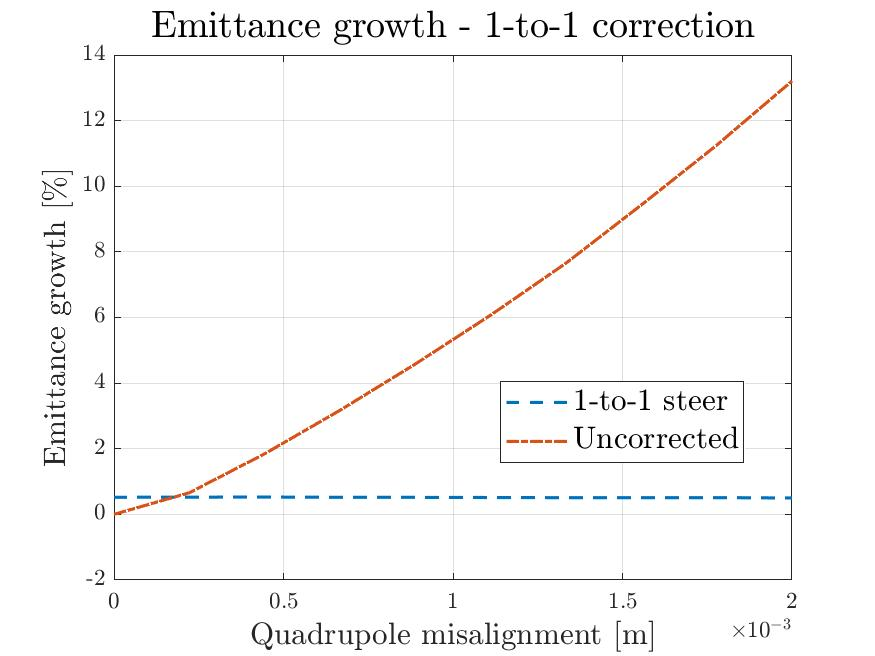
\includegraphics[width=0.65\linewidth, height=0.55\linewidth]{growth_1-to-1_BPM.jpg}
	\caption{Relative emittance growth from the start of the lattice to the end of the lattice as a function of quadrupole misalignment for both uncorrected and 1-to-1 corrected BPM orbits with 1 mm rms BPM misalignment. \label{fig:em_growth_1to1_BPM}}
\end{figure} 

\subsubsection*{5)}
Now we will use dispersion-free steering (DFS) which should give less emittance growth than steering through the centers of the BPMs. In Figure \ref{fig:DFS_orbit} we see a plot of the uncorrected and DFS corrected BPM orbits with both 1 mm rms quadrupole and BPM misalignments. There we see that the BPM orbit for the DFS correction changes less than the uncorrected, but not as little as the 1-to-1 correction in Figure \ref{fig:1-to-1_BPM_orbit}. 

\begin{figure}[htbp!]
	\centering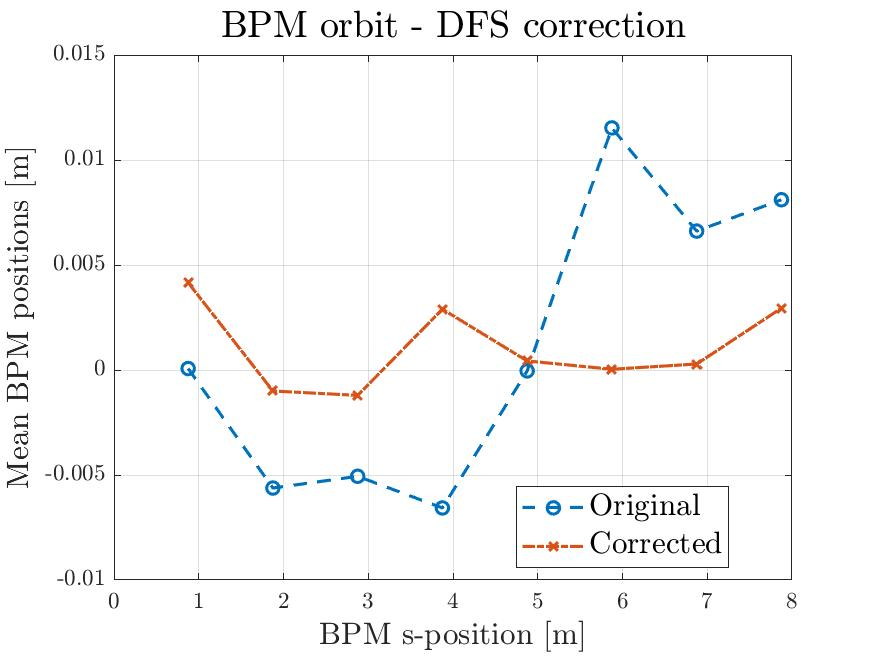
\includegraphics[width=0.65\linewidth, height=0.55\linewidth]{DFS-orbits.jpg}
	\caption{BPM orbits of the beam for uncorrected and DFS corrected BPM orbits with 1 mm rms quadrupole and BPM misalignments. \label{fig:DFS_orbit}}
\end{figure} 

\subsubsection*{6)}
In Figure \ref{fig:em_growth_DFS} we see a plot of the emittance growth as a function of the quadrupole misalignment for both uncorrected and DFS corrected BPM orbits. The DFS corrected orbit gives a much smaller emittance growth as the quadrupole misalignment increases, but is not as low as the 1-to-1 corrected orbit in Figure \ref{fig:em_growth_1to1_BPM}, which is not exactly what we expected. We expected initially that the emittance growth with the DFS correction should be better than the 1-to-1 correction. The emittance growth with the DFS correction is lower than the 1-to-1 correction up until around 1.4 mm quadrupole misalignment, after that the DFS correction gives higher emittance growth. Since the emittance growth with the DFS correction is not always better than the 1-to-1 correction when we increase the quadrupole misalignment, this might be an indication that there is something wrong with the DFS correction code.

\begin{figure}[t!]
	\centering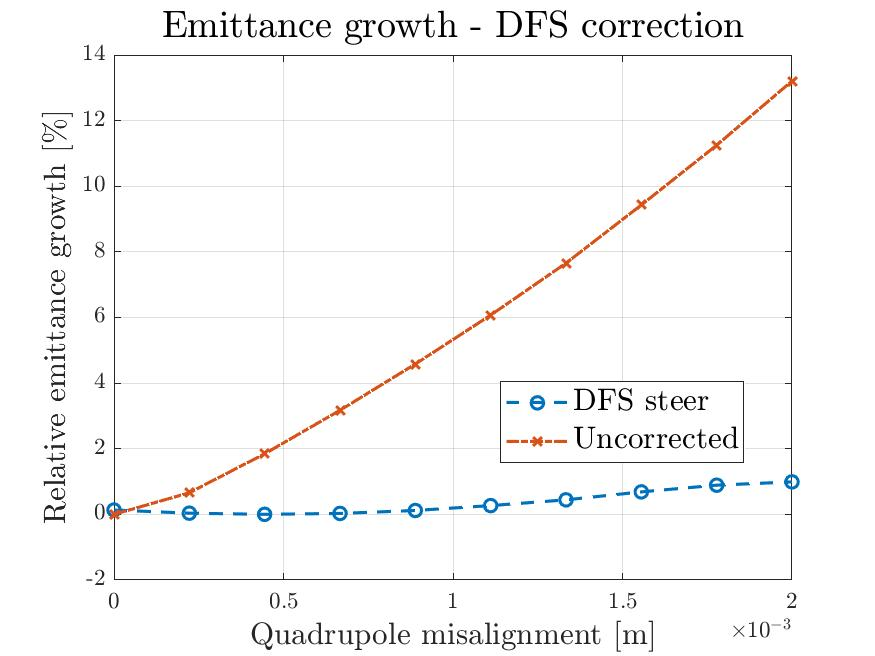
\includegraphics[width=0.65\linewidth, height=0.55\linewidth]{growth_DFS.jpg}
	\caption{Relative emittance growth from the start of the lattice to the end of the lattice as a function of quadrupole misalignment for both uncorrected and DFS corrected BPM orbits with 1 mm rms BPM misalignment. \label{fig:em_growth_DFS}}
\end{figure} 
\newpage
\subsubsection*{7)}
In Figure \ref{fig:em_growth_all} we see a plot of the emittance growth as a function of BPM misalignment for uncorrected, 1-to-1 and DFS corrected BPM orbits. There we see that we get the lowest emittance growth when we use DFS correction, which is constant, as a function of the BPM misalignment (around 0.18\% emittance growth). The emittance growth for the uncorrected orbit also stays constant (around 5.3\%) when the BPM misalignment increases, which is higher than the DFS corrected orbit. The 1-to-1 corrected orbit emittance growth increases almost linearly as the misalignment increases, and becomes very quickly higher than the DFS corrected orbit. After around 5 mm rms BPM misalignment, the 1-to-1 emittance growth becomes higher than for the uncorrected orbit. So the DFS correction seems to give the lowest emittance growth as a function of the BPM misalignment.

\begin{figure}[t!]
	\centering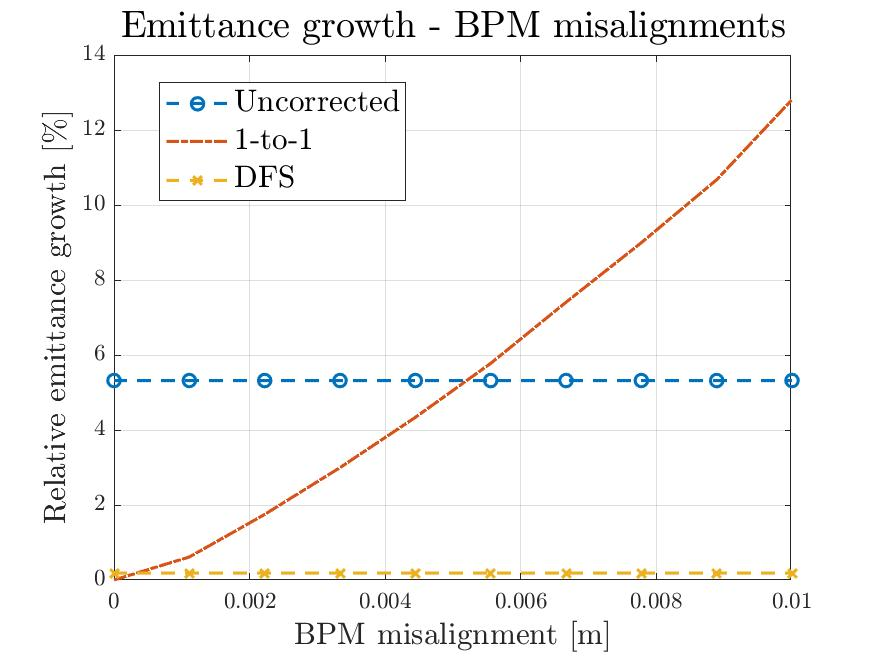
\includegraphics[width=0.75\linewidth, height=0.65\linewidth]{growth_all_BPM.jpg}
	\caption{Relative emittance growth from the start of the lattice to the end of the lattice as a function of BPM misalignment for both uncorrected, 1-to-1 and DFS corrected BPM orbits with 1 mm rms quadrupole misalignment. \label{fig:em_growth_all}}
\end{figure} 

\end{document}
